\section{Resultados}

  \par En esta sección se presentarán resultados de las simulaciones realizadas. Se realizarán histogramas
  comparativos entre las distintas simulaciones. Dichos gráficos serán explicados y analizados brevemente en esta
  sección y con mayor detalle en la siguiente.

  \par Como comentario general de los histogramas, vale aclarar que se proyectará sobre el eje de las abcisas la
  durabilidad del sistema en meses. Mientras que en el eje de las ordenadas al origen graficaremos las frecuencias
  relativas de los valores obtenidos por la simulación.

  \par Cabe recordar, los valores de las variables para la simulación mediante los algoritmos anteriormente descritos,
  para cada uno de los problemas ya mencionados.

  \begin{itemize}
    \item \underline{Simulación 1:} 5 máquinas en funcionamiento, 2 máquinas de repuesto y 1 operario, i.e,
    $N = 5, \; S = 2, \; T_F = 1, \; T_R = 1/8, \; Op = 1$
    \item \underline{Simulación 2:} 5 máquinas en funcionamiento, 2 máquinas de repuesto y 2 operario, i.e,
    $N = 5, \; S = 2, \; T_F = 1, \; T_R = 1/8, \; Op = 2$
    \item \underline{Simulación 3:} 5 máquinas en funcionamiento, 3 máquinas de repuesto y 1 operario, i.e,
    $N = 5, \; S = 3, \; T_F = 1, \; T_R = 1/8, \; Op = 1$
  \end{itemize}

  \pagebreak
  \subsection{\underline{Comparación 1:} Simulaciones 1 y 2}

    \par En el gráfico sucesor se realiza una comparación entre las dos primeras simulaciones, donde en una de ellas
    se simula con un solo operario, mientras que en la otra se simula con dos.

    \begin{figure}[H]
      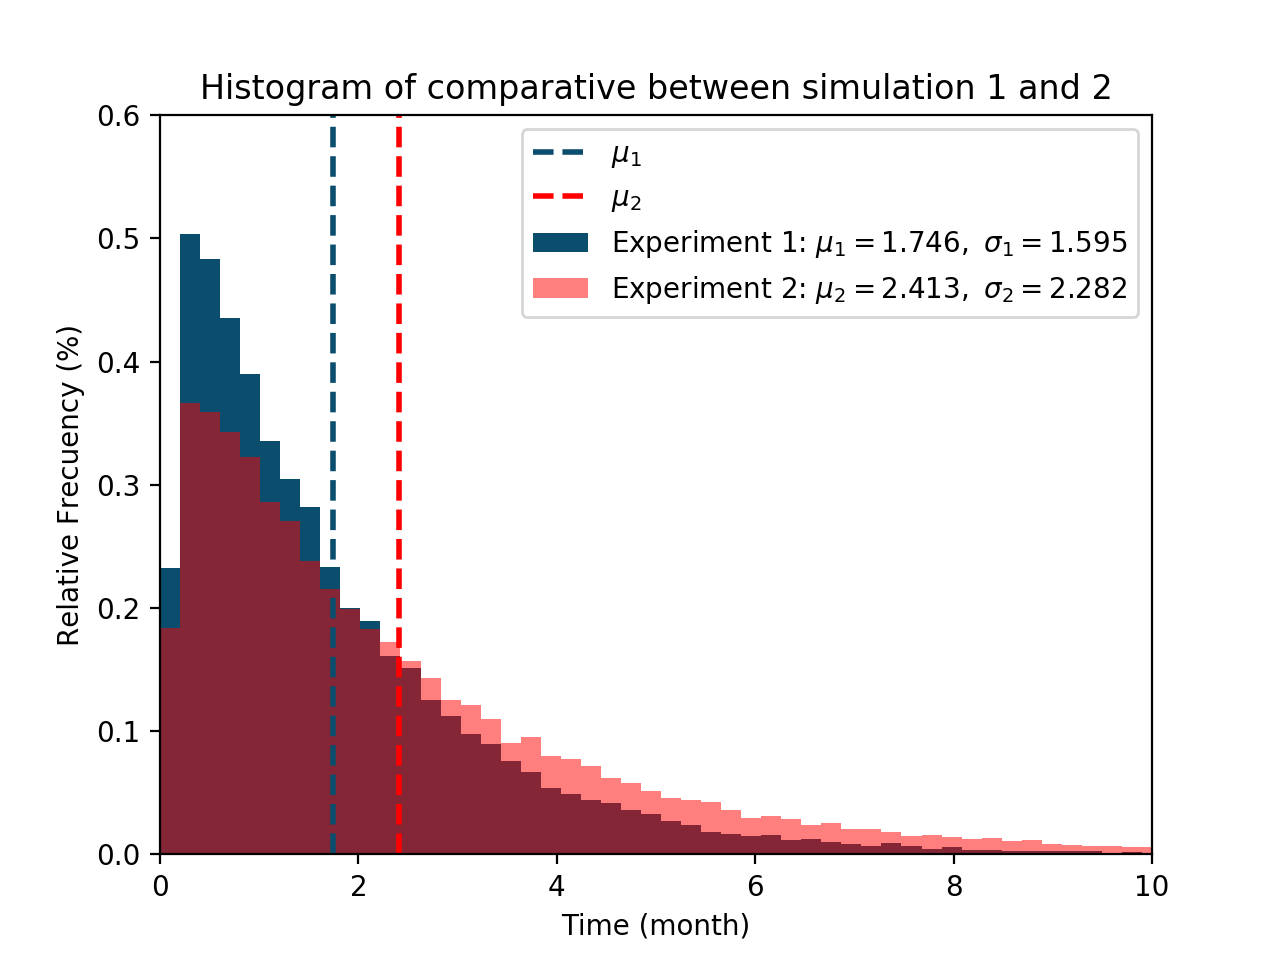
\includegraphics[scale=1.1]{graphics/Comparative_graphic_1.png}
      \caption{Comparación simulaciones 1 y 2}
      \centering
    \end{figure}

    \par Podemos apreciar en la \textit{Figura 1} que existe una ganancia aproximada de un mes de la simulación con un
    operario más sobre la representación del sistema incial. Dicho resultado es el esperado, dado que la velocidad de
    reparación de una máquina es mayor pues aumenta la cantidad de trabajadores encargados de dicha tarea.

  \pagebreak
  \subsection{\underline{Comparación 2:} Simulaciones 1 y 3}

    \par Al igual que en la comparación anterior, el objetivo del siguiente gráfico entre el sistema original y la
    simulación con una máquina de repuesto más, es dejar en evidencia cual es la mejoría, en caso que existiese, en el
    agregado de un operario en el sistema de la lavandería.

    \begin{figure}[H]
      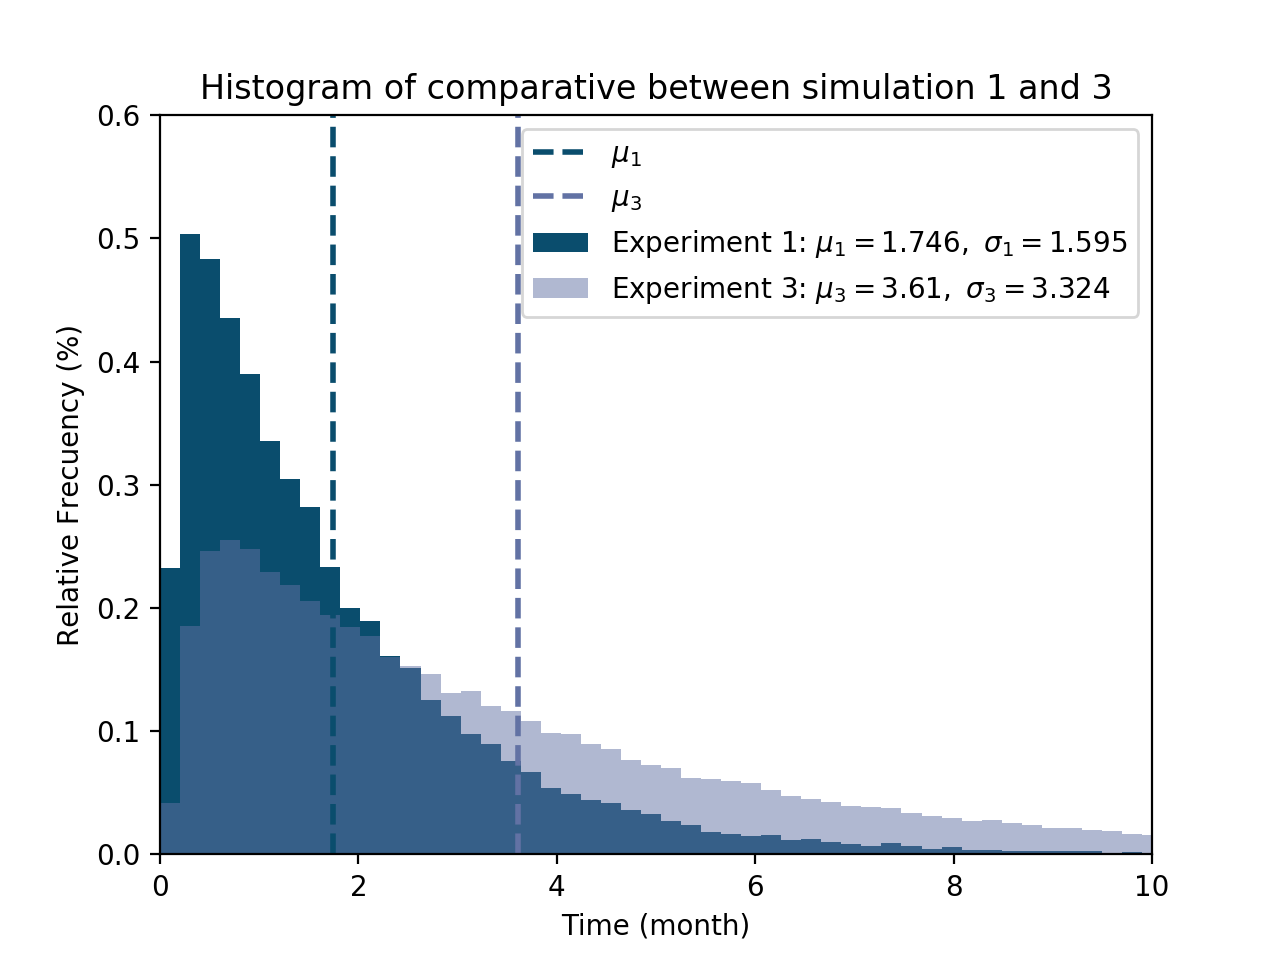
\includegraphics[scale=1.1]{graphics/Comparative_graphic_2.png}
      \caption{Comparación simulaciones 1 y 3}
      \centering
    \end{figure}

    \vspace{5mm}
    \par Similarmente a los ocurrido en la comparación anterior, se puede apreciar una mejoría de la simulación con una
    máquina de repuesto más, sobre la representación del sistema inicial. Dicha mejoría es aún mayor que en la anterior
    comparación, dado que este mismo suceso ocurre con los valores esperados de las simulaciones, es decir, la
    esperanza del segundo sistema es mayor que la del primero. Numéricamente esta diferencia ronda los dos meses.
    Nuevamente, este resultado es el esperado, dado que en el momento que ocurriese un fallo en alguna de las máquinas,
    se contará con un repuesto más que en sistema inicial.

  \pagebreak
  \subsection{\underline{Comparación 3:} Simulaciones 2 y 3}

    \par En el esquema correlativo, podemos apreciar las diferencias existentes entre las dos posibles soluciones a la
    mejora del sistema original. Es decir, se comparan los histogramas resultantes de las
    simulaciones con dos máquinas de repuesto y un operario contra tres máquinas y un operario.

    \begin{figure}[H]
      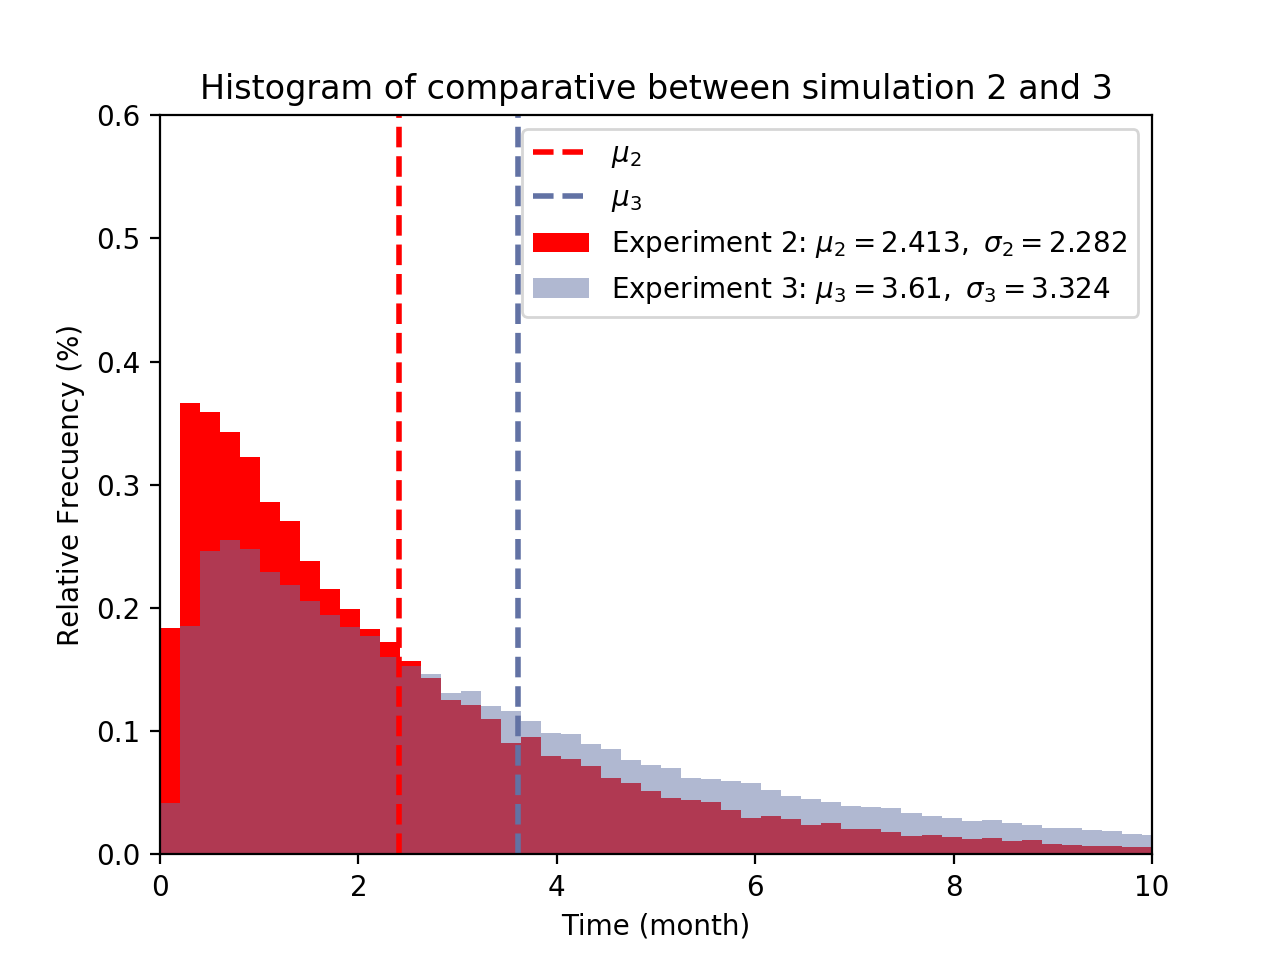
\includegraphics[scale=1.1]{graphics/Comparative_graphic_3.png}
      \caption{Comparación simulaciones 2 y 3}
      \centering
    \end{figure}

    \par Dado que, como se observo en las \textit{Figura 1} y \textit{Figura 2}, existe una diferencia cercana al mes
    entre los valores de las simulaciones con uno y dos operarios, y de dos meses entre las representaciones con dos y
    tres máquinas de repuesto, este histograma muestra una desigualdad cercana al mes entre los tiempos de vida
    esperados de dichas simulaciones.

  \pagebreak
  \subsection{\underline{Extrapolación en 3D}}

    \par Por último, el siguiente figura, realizado en tres dimesiones, tiene como objetivo acentuar las conclusiones
    ya realizadas en las secciones y gráficos anteriores, esto es, dejar en evidencia que en ambos casos, es decir,
    agregando ya sea operarios o máquinas el sistema mejorará, pero dicha mejora será aún mayor en la simulación que
    adicione máquinas.

    \begin{figure}[H]
      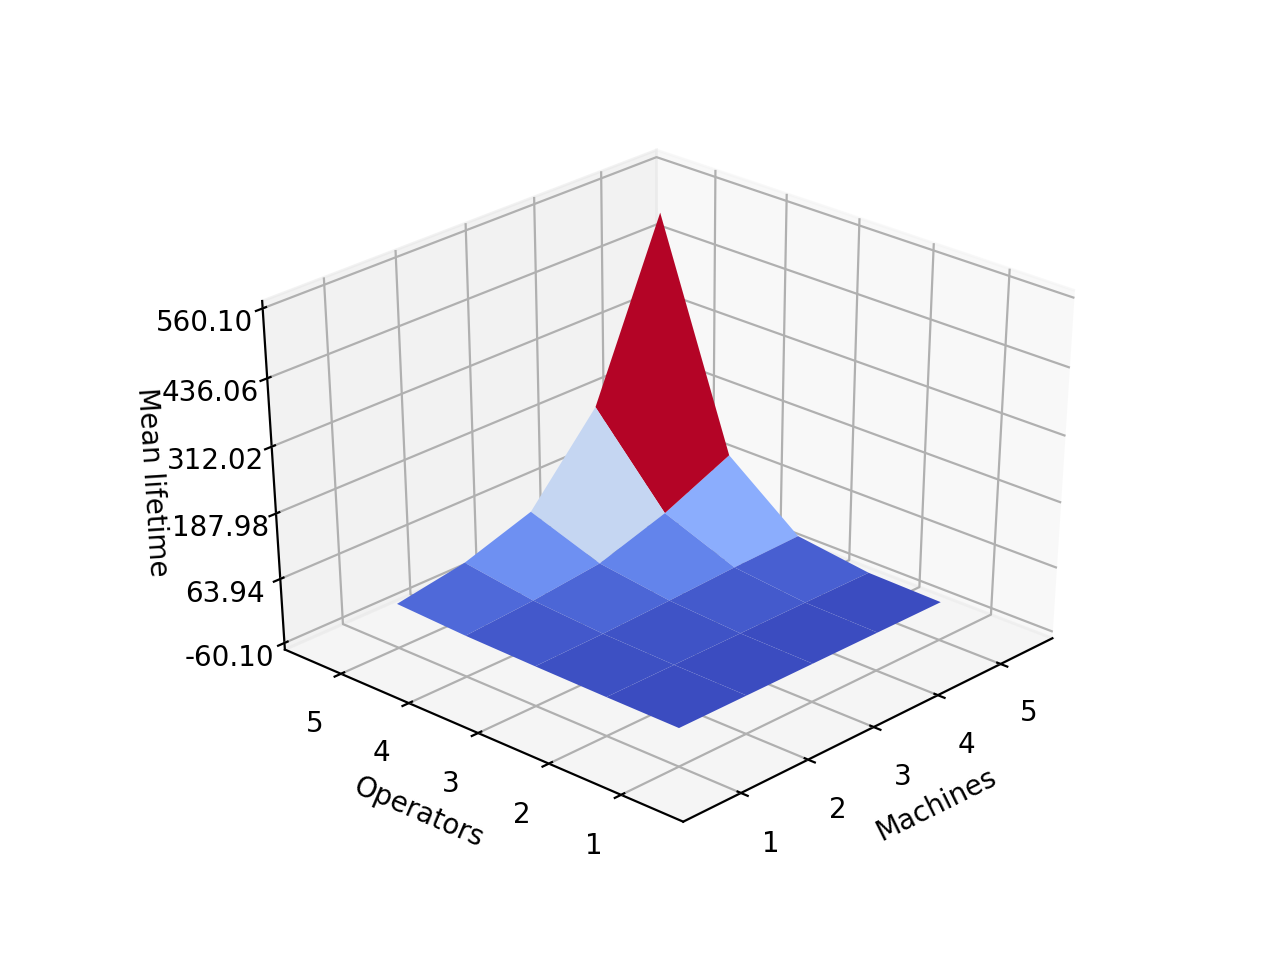
\includegraphics[scale=1.2]{graphics/Figure_4.png}
      \caption{Simulación en 3D}
      \centering
    \end{figure}

  \pagebreak
  \subsection{Tablas comparativas entre simulaciones}

    \par Los consecuentes resultados pertenecen a los tres sistemas simulados y recientemente desarrollados. Dichos
    valores se corresponden con un intervalo de confianza del 99 \%.

    \begin{itemize}
      \item \textbf{Figura 1: 5 máquinas funcionando, 2 máquinas de repuesto y 1 operario}
        \begin{center}
          \begin{tabular}{| l | l | l | l |}
          \hline
            Confianza & $\mu$ & $\sigma^2$ & $\sigma$ \\\hline\hline
            99 \% & 1.746 & 2.545 & 1.595 \\\hline
          \end{tabular}
        \end{center}
      \vspace{5mm}
      \item \textbf{Figura 2: 5 máquinas funcionando, 2 máquinas de repuesto y 2 operarios}
        \begin{center}
          \begin{tabular}{| l | l | l | l |}
          \hline
            Confianza & $\mu$ & $\sigma^2$ & $\sigma$ \\\hline\hline
            99 \% & 2.413 & 5.208 & 2.282 \\\hline
          \end{tabular}
        \end{center}
      \vspace{5mm}
      \item \textbf{Figura 3: 5 máquinas funcionando, 3 máquinas de repuesto y 1 operario}
        \begin{center}
          \begin{tabular}{| l | l | l | l |}
          \hline
            Confianza & $\mu$ & $\sigma^2$ & $\sigma$ \\\hline\hline
            99 \% & 3.610 & 11.049 & 3.324 \\\hline
          \end{tabular}
        \end{center}
    \end{itemize}
